% !TeX encoding = UTF-8
% !TeX program = xelatex
% !TeX spellcheck = en_US

\documentclass[twosides]{article}

\usepackage{geometry}
\geometry{paperwidth=420mm,paperheight=297mm,left=0cm,right=0cm,top=.5cm,bottom=0cm}

\usepackage[PunctStyle=kaiming]{xeCJK}
\setCJKmainfont[Path=../fonts/,BoldFont=NotoSansCJKsc-Bold.otf]{NotoSansCJKsc-DemiLight.otf}
\setmainfont[Path=../fonts/,BoldFont=NotoSansCJKsc-Bold.otf]{NotoSansCJKsc-DemiLight.otf}
\newfontfamily{\Acumin}[Path=../fonts/]{AcuminExtraCondSemibold.otf}

\usepackage{xcolor}
\definecolor{lightblue}{HTML}{31c6f4}
\definecolor{darkblue}{HTML}{1f6899}

\usepackage{tikz}

\long\def\MakeCover#1#2#3#4{
    \def\halfthk{#1*0.025mm}
    \clearpage
    \begin{center}
        \begin{tikzpicture}
            \node[anchor=north west,inner sep=0] at (\halfthk-10mm,10mm) {
\includegraphics[width=175mm]{src/front.pdf}};
            \node[anchor=north east,inner sep=0] at (-\halfthk+10mm,10mm) {
\includegraphics[width=175mm]{src/back.pdf}};
            \node[anchor=north,inner sep=0] at (0mm,10mm) {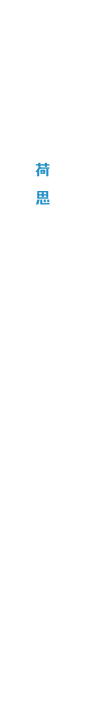
\includegraphics[width=30mm]{src/ridge.pdf}};
            
            \node[scale=3.67,white] at (\halfthk+77mm,-151mm) {\Acumin #2};
            \node[scale=3.67,white] at (\halfthk+77mm,-164mm) {\Acumin #3};
            \node[darkblue] at (-\halfthk-77.5mm,-174mm) {\parbox{75mm}{#4}};
            \node[anchor=north,darkblue,scale=1.6] at (0mm,-145mm) {\rotatebox{-90}{\Acumin #2}};
            \node[anchor=north,darkblue,scale=1] at (0mm,-155.7mm) {年};
            \draw[darkblue] (-2.5mm,-165mm) -- (2.5mm,-165mm);
            \node[anchor=north,darkblue,scale=1] at (0mm,-169.5mm) {第};
            \node[anchor=north,darkblue,scale=1.6] at (0mm,-173.2mm) {\rotatebox{-90}{\Acumin #3}};
            \node[anchor=north,darkblue,scale=1] at (0mm,-179.7mm) {期};

            \fill[lightblue] (-165mm-\halfthk,10mm)--(165mm+\halfthk,10mm)--(165mm+\halfthk,-10mm)--(-165mm-\halfthk,-10mm);
            \fill[darkblue] (-165mm-\halfthk,-245mm)--(165mm+\halfthk,-245mm)--(165mm+\halfthk,-225mm)--(-165mm-\halfthk,-225mm);

            \draw[thick]
                (-180mm-\halfthk,0mm)--(-170mm-\halfthk,0mm)
                (180mm+\halfthk,0mm)--(170mm+\halfthk,0mm)
                (-180mm-\halfthk,-235mm)--(-170mm-\halfthk,-235mm)
                (180mm+\halfthk,-235mm)--(170mm+\halfthk,-235mm)
                (-155mm-\halfthk,25mm)--(-155mm-\halfthk,15mm)
                (155mm+\halfthk,25mm)--(155mm+\halfthk,15mm)
                (-155mm-\halfthk,-260mm)--(-155mm-\halfthk,-250mm)
                (155mm+\halfthk,-260mm)--(155mm+\halfthk,-250mm)
                (-\halfthk,25mm)--(-\halfthk,15mm)
                (\halfthk,25mm)--(\halfthk,15mm)
                (-\halfthk,-260mm)--(-\halfthk,-250mm)
                (\halfthk,-260mm)--(\halfthk,-250mm); 
            % \draw (-\halfthk, 0mm) rectangle (\halfthk, -235mm);
            % \draw (-155mm-\halfthk, 0mm) rectangle (155mm+\halfthk, -235mm);
            % \draw (-165mm-\halfthk, 10mm) rectangle (165mm+\halfthk, -245mm);
        \end{tikzpicture}
    \end{center}
}
\def\fr{\mathfrak}
\def\det{\mathrm{det}}
\def\={\mathop{=}}
\def\rk{\mathrm{rk}}
\def\bar{\overline}
\def\check{\widecheck}
\def\hat{\widehat}
\def\bl{\textcolor{blue}}

\newcommand\dif{\mathop{}\!\mathrm{d}}  % 微分符号
\newcommand\real{{\mathbf{R}}}  % 实数集
\newcommand\abs[1]{\lvert#1\rvert}
\newcommand\VECTOR{\symbf}  % 向量
\newcommand\MATRIX{\symbf}  % 矩阵
\newcommand\vn{{\VECTOR{n}}}
\newcommand\vx{{\VECTOR{x}}}
\newcommand\mA{{\MATRIX{A}}}
\newcommand\mK{{\MATRIX{K}}}

\DeclareRobustCommand\cs[1]{\texttt{\char`\\#1}}
\providecommand\pkg[1]{{\sffamily#1}}

\usepackage{enumitem}
\setlist[enumerate, 1]{label=(\arabic*)}

\addbibresource{ref/refs.bib}

\begin{document}

\title{Ricci-Flat Metrics on Some K3\\ Surfaces Admitting Elliptic Fibrations}
\author{Zhang Ruitong\footnote{张睿桐,清华大学数学系数 72 班.}}

% !TeX root = ../thuthesis-example.tex

% 中英文摘要和关键字

\begin{abstract}
 卡拉比--丘流形上的里奇平坦度量的具体构造一直是一个重要的问题。在某些特殊的卡拉比--丘流形上,用半平坦度量的渐进估计有一些不错的结果。本文将介绍Hein给出的有理椭圆曲面上半平坦度量构造及估计的一些结果。本文的主要参考文献是Hein的文章\cite{hein2012gravitational}。

  % 关键词用“英文逗号”分隔,输出时会自动处理为正确的分隔符
  \thusetup{
    keywords = {卡拉比--丘流形,半平坦度量,有理椭圆曲面},
  }
\end{abstract}

\begin{abstract*}
The explicit construction of Ricci-flat metric on Calabi--Yau manifolds has been an important question long since. On some special Calabi--Yau manifolds, asymptotics using semi-flat metrics have some well results. We'll introduce some results of Hein on constructing and estimating semi-flat metrics on rational elliptic surfaces in this paper. The main reference is Hein's paper\cite{hein2012gravitational}.

  % Use comma as separator when inputting
  \thusetup{
    keywords* = {Calabi--Yau manifolds, semi-flat metric, rational elliptic surface},
  }
\end{abstract*}


\tableofcontents

% !TeX root = ../Lie.tex


Let's consider an isolated hypersurface singularity $(V,\0)\subset \left(\Cc^n,\0\right)$ defined by a holomorphic function germ $f\in \mathcal O_{\Cc^n,\0}$.
In \cite{MY},  Mather and Yau proved that  the complex structure $(V,\0)$ is determined by one of its analytic invariant, the moduli algebra $A(V)$, which we would also denote by $A(f)$ in this paper.
In \cite{Yau}, Yau considered moreover  the derivation Lie algebra $L(f)$ of $A(f)$, and proved its solvability in \cite{Yau5}. He asked whether $L(f)$ is a complete invariant of the singularity $(V,\0)$.

Motivated by Dimca's theorem 2.2 in \cite{Di}, the generalized moduli algebra $A^*(V)$ and new Lie algebra $L^*(V)$ were also considered in \cite{BN}. Detailed definition of them will be introduced in the next section, subsection \ref{sec-2.4}. Here we just point out that it's obvious from definition that $L^*(f)$ is also determined by the complex structure of  $(V,\0)$. And we can ask again whether the converse is true.

Following the question whether these Lie algebras arising from  singularities are enough to determine the singularities themselves, some inspiring examples were proved in \cite{SY} and \cite{BN}, where the Torelli-type theorem was proved to be valid for some simple elliptic singularities.  But the problem is hard in general, since there is few methods to determine whether two Lie algebras are isomorphic or not. One of such examples was encountered in \cite{BN}, for which only weak Torelli-type theorem was verified. 

However, this approach is also valuable for another purpose: provide a general method to construct non-trivial families of solvable Lie algebras with several parameters, since the classification of solvable and nilpotent Lie algebra remains to be a vast open area. This article, as a continuation of the work in 
\cite{SY} and \cite{BN}, obtains the following main results: 

\begin{theorem}\label{mth1} \hfill
  \item[(1)] The family of hypersurface singularities in $\Cc^3$ defined by  
    \[f=f_\bt\coloneq x^4+y^4+z^4
      +t_1x^2y^2+t_2x^2z^2+t_3y^2z^2
    +t_4x^2yz+t_5xy^2z+t_6xyz^2\]
    give rise to nontrivial $6$-parameter families, $\tilde L^*(f_\bt)$ and $\tilde L(f_\bt)$, of solvable Lie algebras of dimension 37.

  \item[(2)] The family of hypersurface singularities in $\Cc^4$ defined by  
    \begin{align*}
      f=f_\bt\coloneq
        & x^4+y^4+z^4+w^4
        +t_1x^2y^2+t_2x^2z^2+t_3x^2w^2+t_4y^2z^2+t_5y^2w^2 \\
        &+t_6z^2w^2+t_7x^2yz+t_8xy^2z+t_9xyz^2
        +t_{10}x^2yw+t_{11}xy^2w \\
        &+t_{12}xyw^2+t_{13}x^2zw+t_{14}xz^2w+t_{15}xzw^2
        +t_{16}y^2zw\\
        &+t_{17}yz^2w+t_{18}yzw^2+t_{19}xyzw
    \end{align*}
    give rise to $19$-parameter families, $\tilde L^*(f_\bt)$ and $\tilde L(f_\bt)$, of solvable Lie algebras of dimension 106.
\end{theorem}

The verification of nontriviality of the $19$-parameter families encountered obstacles due to technical reason, but some other non-trivial families of Lie algebras are given by the way. 

The structure of this article is as follows. In section \ref{sec2}, we collect the definitions and facts mentioned above which are necessary for the latter sections. Relevant materials can be found in \cite{BN} and \cite{GL}. In section \ref{sec3}, we demonstrate the computation of  $L(f_\bt)$ and $L^*(f_\bt)$ arising from the singularities defined by $f_\bt$, a homogeneous polynomial with parameters $\bt\in \Cc^m$. In section \ref{sec4}, we recall the definition of ``liftable Lie algebra'', which follows from the definition 2.2 in \cite{SY}, in order to make the verification of Theorem \ref{mth1}  realizable for a computer.

% !TeX root = ../Lie.tex

Now start from a convergent power series $f\in \m \subset \Cc\{\xn\}=\Cc\{x_1,\cdots, x_n\}$, where $\m = \lan x_1,\cdots, x_n\ran$ is the unique maximal ideal of $\Cc\{x_1,\cdots,x_n\}$, the local ring of convergent power series of $n$ variables, which can also be regarded as the coordinate ring of the complex space germ $(\Cc^n,\0)$. Then the origin of $\Cc^n$ lies in the hypersurface $\{ f = 0\} \subset \Cc^n$.

\subsection{Isolated hypersurface singularities} Let $V=V(f)$ denote the germ of $\{f=0\}$ at the origin of $\Cc^n$. Since the singular locus of $V$ is exactly where the gradient of $f$ vanishes, we say $V$ is a germ of isolated hypersurface singularity if the origin $\0\in \Cc^n$  is an isolated point of 
$$\left\{f=0,\pd f{x_1}=0,\cdots, \pd f{x_n}=0\right\}.$$
In this case we also say $f$ defines a isolated hypersurface singularity $V$.

\subsection{Moduli algebra}\label{sec-2.2}
For $f\in \m$, we introduce its Jacobian ideal to be 
\[j(f)\coloneq \lan \pd f{x_1},\cdots, \pd f {x_n}\ran.\]
and its Tjurina algebra to be 
\[A(f)\coloneq  \Cc\{\xn\} / \lan f, j(f)\ran.\]
According to lemma 2.3 of \cite[113]{GL}, $A(f)$ is of finite dimension iff $f$ defines an isolated hypersurface singularity. This algebra is also said to be  moduli algebra of $V=V(f)$. The well-known Mather--Yau theorem states that 

\begin{theorem}[\cite{MY}]\label{MY}
  For  isolated hypersurface singularities $V(f_1), V(f_2)$ defined by $f_1,f_2\in \m\subset \Cc\{\xn\}$, they are isomorphic as complex space germs if and only if their moduli algebras $A(f_1)$ and $A(f_2)$ are isomorphic as $\Cc$-algebras.
\end{theorem}
Consequently, the moduli algebra $A(f)$ is a complete invariant of the isolated hypersurface singularities $V(f)$. 


\subsection{Yau algebra}\label{sec-2.3}
Suppose we have a homomorphism of $\Cc$-algebras  $A\to B$, which is equivalent to say that $B$ is an $A$-algebra.  Denote $\Endo_A B$ the endomorphisms of $B$ as an $A$-module, then we can define the $A$-derivation algebra of $B$ to be the submodule
\[\Der_A B=\{ \delta \in \Endo_A B\,\mid \delta(fg)= \delta(f)g+f\delta(g), \forall f,g \in B\},\]
whose Lie bracket is the commutator of linear endomorphisms. We would consider  the case $A=\Cc$ before section \ref{sec4}, and then the case $A=\Cc\{t\}$ or $\Cc\{\bt\}=\Cc\{t_1,\cdots, t_m\}$ will also be taken into consideration.
\begin{remark}
  To obtain
  \[\Der_\Cc \Cc\{\xn\} = \bigoplus_{i=1}^n\Cc\{\xn\} \pd{}{x_i},\]
  one may need moreover that the derivation over $\Cc\{\xn\}$ is continuous with respect to the $\m$-adic topology. However, this doesn't make any difference when $B$ is also a  finite generated module over $A$. This is the most case we consider. 
\end{remark}

The Tjurina algebra $A(f)$ for $f\in \m$ is a $\Cc$-algebra, so we now can introduce its derivation Lie algebra as
\[L(f)\coloneq  \Der_\Cc A(f).\]
Motivated by Theorem \ref{MY}, we can ask whether  $L(f)$ is also a complete invariant of the isolated hypersurface singularities $V(f)$.	

\subsection{New Lie algebra}\label{sec-2.4}
In \cite{BN}, a new complete invariant of quasi-homogeneous isolated hypersurface singularities $V=V(f)$ was defined as
\[A^*(f)\coloneq \Cc\{\xn\}/\lan f, j(f), H(f)\ran,\]
where
\[H(f)\coloneq \det  \left( \frac{\partial^2 f}{\partial x_i \partial x_j}\right)_{1\leqslant i,j \leqslant n } \]
is the Hessian of $f$. Consequently, another Lie algebra $L^*(f)\coloneq \Der_\Cc A^*(f)$ called new Lie algebras in \cite{BN} arises from the singularity defined by $f$, and a question similar to $L(f)$ can be proposed.

Before the concrete computation in section \ref{sec3}, we present the following results about the grading structure of the above algebras, which can be found in \cite{BN}:	
\begin{proposition}[\cite{BN}]\label{res}
  Let $f\in \Cc\{\xn\}$ be a homogeneous polynomial of degree $d\geqslant 2$ defining an isolated hypersurface singularity in $( \Cc^n, \0)$.
  Note that there are natural grading which can be denoted to be 
  \begin{align*}
    A(f)=\bigoplus_{k=0}^DA(f)_k,&
    A^*(f)=\bigoplus_{k=0}^{D^*}A^*(f)_k.
  \end{align*}
  \item[(1)](Theorem 2.3, Proposition 2.1)  The degree-$D$ part of $A(f)$ is $1$-dimensional with a basis represented by $H(f)$. In particular, $D\coloneq  \deg  H(f) = n(d-2)$ . Moreover, the total dimension of $A(f)$ is  $ (d-1)^n.$
  \item[(2)](Theorem 2.3) The natural projection $A(f) \to A^*(f)$ induces isomorphisms of $\Cc$-linear spaces $A(f)_k\stackrel \sim \to A^*(f)_k, 0 \leqslant k \leqslant D-1$. In particular, $D^*=D-1$. Moreover, the total dimension of $A^*(f)$ is  $ (d-1)^n-1.$
  \item[(3)](Corollary 2.1) $L(f)$  is solvable, while $L^*(f)$ is solvable given $d\geqslant 4$.
  \item[(4)](Remark 6.1) $L(f)$ and $L^*(f)$ are naturally graded with no negative part and share the same total dimension.
  \end{proposition}
  We also denote $\Cc\{\xn\}_k$ to be  the degree $k$-part of $\Cc\{\xn\}$, i.e., the vector space consists of homogeneous polynomials of degree $k$, then we have $\forall K \geqslant 0$, 
  \[\Cc\{\xn\} = \left( \bigoplus_{k=0}^K \Cc\{\xn\}_k \right)\oplus \m^{K+1}\]
  as $\Cc$-vector space.

  %	\[
  %	\Cc\{\xn\}=\overline{\bigoplus_{k\geqslant 0}\Cc\{\xn\}_k},\]
  %	where the closure is taken with respect to the $\m$-adic topology of $\Cc\{\xn\}$. 

% !TeX root = ../thuthesis-example.tex

\section{Metric on complex torus bundle}
In this section, we discuss some important notions to express the local model of an elliptic fibration explicitly. In this process, we need to choose local trivialization properly and consider the monodromy. We then give a explicit formula of a semi-flat metric using the coordinates obtained by period map.
\subsection{Local model}
In this subsection, we discuss the local model, and explain how a metric will be constructed.
\begin{definition}
For an elliptic fibration, we call a metric semi-flat
if it restricts to a flat metric on each fiber.
\end{definition}
Let $f\colon X\rightarrow \mathbb{P}^1$ be a holomorphic submersion such that all fibers $X_p=f^{-1}(p)$ are complex torus, and suppose $f$ admits a holomorphic section $\sigma$ with a 2
-form $\omega$, which restricts to a K{\"a}hler form on each fiber $X_p$ and there exists $c_i\in\mathbb{R}$ and $\xi_i(p)\in H^2(X_p,\mathbb{Z})$ such that
\[ [\omega|_{X_p}]=\sum_i c_i\xi_i(p),\qquad  \forall p\in\mathbb{P}^1 \;. \]
\indent For $\epsilon>0$ and $p\in\mathbb{P}^1$, from Yau's result \cite{yau1978ricci}, there exist a unique Ricci-flat K{\"a}hler metric $g_{p,\epsilon}$ with $\operatorname{Vol}(X_p,g_{p,\epsilon})=\epsilon$ whose K{\"a}hler class is $[\omega|_{X_p}]$. Restricting $g_{p,\epsilon}$ to $T_{\sigma(p)}X_p$ then induces a Hermitian fiber metric $h_\epsilon$ on the holomorphic vector bundle $E\\coloneq \sigma^*T_{X/\mathbb{P}^1}$ over $\mathbb{P}^1$.\\ \indent
Suppose $X$ admits a holomorphic volume form $\Omega$. There exists a unique Riemannian metric $g_{\mathbb{P}^1,\epsilon}$, compatible with the complex structure of $\mathbb{P}^1$, and the faithful pairing 
\[ E\otimes T^{1,0}\mathbb{P}^1\rightarrow \mathbb{C} \]
induced by $h_\epsilon$ and $g_{\mathbb{P}^1,\epsilon}$ is isometric to the one induced by $\Omega$.\\ \indent
We can choose a fibre-preserving biholomorphism $X\simeq E/\Lambda$ for a holomorphic lattice bundle $\Lambda\subset E$. Thus $\Lambda$ induces a flat $\mathbb{R}$-linear connection on $E$, thus we can define an integrable horizontal distribution $\mathscr{H}$ on $X$. Then define
\[ g_{\mathrm{sf},\epsilon}(u,v)=g_{p,\epsilon}(Pu,Pv)+g_{\mathbb{P}^1,\epsilon}(df(u),df(v)) \]
for $u,v\in T_xX$, where $P$ is the projection along $\mathscr{H}_x$.\\ \indent
Now we see the metric locally, thus we choose a local trivialization on an open subset $U$ of $\mathbb{P}^1$, thus we have
\[ X|_U\simeq E|_U/\Lambda \simeq(U\times \mathbb{C})/\Lambda \; , \]
denote the coordinate $z$ on $U$ and $w$ on the $\mathbb{C}$.
Fix an oriented basis $\{\tau_1,\tau_2\}$ for $\Lambda$ at a generic point, and extend it to $\tau_i\in \mathscr{O}(U,\mathbb{C})$ that generate the lattice everywhere and let $(\xi^1,\xi^2)$ be $\mathbb{R}$-dual to $(\tau_1,\tau_2)$. The assumption we made before means the existence of a matrix $Q\in M_{2\times2}(\mathbb{R})$, $Q+Q^T=0$, such that
\[ \omega=\frac{1}{2}Q_{ij}\xi^i\wedge\xi^j \]
restricts to K{\"a}hler metric on each fiber. Define $T\in \mathscr{O}(U,M_{1\times2}(\mathbb{C}))$ by
\[ \tau_1=T_{11}\qquad \tau_2=T_{12}\; . \]
\indent Consider the monodromy, we have a matrix $A\in GL(2,\mathbb{R})$, then $A^TQA=Q$. There exists $S\in GL(2,\mathbb{R})$, unique up to right multiplication by a matrix in $Sp(2,\mathbb{R})$ such that \[S^TQS=\begin{pmatrix}
0 & 1\\
-1 & 0
\end{pmatrix}\; .\]
\\ \indent We thus write $TS=(R,RZ)$ with multivalued holomorphic maps $R\colon U\rightarrow \mathbb{C}$ and $Z\colon U\rightarrow \mathbb{C}$. By Griffiths--Harris \cite{griffiths1978principles}, $\omega$ being positive $(1,1)$ is equivalent to the image of $Z$ is contained in upper-half plane. And we have
\[ \omega=iH dw\wedge d\bar{w}\; , \]
and
\[ H^{-1}\\coloneq 2|R|^2\operatorname{Im}  Z=i\bar{T}Q^{-1}T\; . \]
\indent Here $Z$ is actually the so called period map, although actually is not well-defined since $S$ is only unique up to multiplication by matrix in $\operatorname{Sp}(2,\mathbb{R})$. The flat connection induced before has Christoffel symbol
\[\Gamma(z,w)=\frac{\partial T}{\partial z}\begin{pmatrix}
T \\
\bar{T}
\end{pmatrix}^{-1}\begin{pmatrix}
w\\
\bar{w}
\end{pmatrix}\in\mathbb{C}\; .\]

\subsection{Construction of metric}
In this subsection, we give explicit formula for a semi-flat metric constructed by Hein \cite{hein2012gravitational}.
\begin{lemma}
For $H$ as defined above and $\epsilon>0$, denote $\displaystyle H(\epsilon)=\frac{\epsilon}{\sqrt{\det Q}}H$, if $\Omega=gdz\wedge dw$ where $g$ is holomorphic, then the K{\"a}hler form of $g_{\operatorname{sf},\epsilon}$ is
\[ \omega_{\mathrm{sf},\epsilon}=i|g|^2H(\epsilon)^{-1}dz\wedge d\bar{z}+iH(\epsilon)(dw-\Gamma dz)\wedge(d\bar{w}-\bar{\Gamma}d\bar{z})\; . \]
It is a closed form whose top power is $2\Omega\wedge\bar{\Omega}$, so is Calabi--Yau.
\end{lemma}
\begin{lemma}
Using the above notations, the metric $g_{\mathbb{P}^1,\epsilon}$ on the base are K{\"a}hler, and has Ricci form 
\[ \rho(\omega_{\mathbb{P}^1,\epsilon})=-i\partial\bar{\partial}\log(\operatorname{Im} Z)=\frac{i dZ\wedge d\overline{Z}}{4(\operatorname{Im} Z)^2}\; . \]
\end{lemma}
\begin{proof}
  First notice that \[ |R|^2\operatorname{Im} Z=\frac{1}{H}\; ,\]
and notice that Ricci form is invariant under scalar multiplication on metric. Then denote \[ f=\operatorname{Im} Z=\frac{1}{2i}(Z-\bar{Z})\; . \]
\indent Then we have
\begin{displaymath}
\begin{split}
\partial\bar{\partial}\log(\operatorname{Im} Z)&=\partial\left(\frac{f_{\bar{z}}}{f}d\bar{z}\right)\\
&=\frac{ff_{z\bar{z}}-f_z f_{\bar{z}}}{f^2}dz\wedge d\bar{z}\\
&=\frac{Z_z\bar{Z}_{\bar{z}}}{(Z-\bar{Z})^2}dz\wedge d\bar{z}\\
&=\frac{-|Z_z|^2}{4(\operatorname{Im} Z)^2}dz\wedge d\bar{z}\; .
\end{split}
\end{displaymath}
\indent And notice that 
\[ dZ\wedge d\bar{Z}=Z_zdz\wedge\overline{Z_z}d\bar{z}=|Z_z|^2dz\wedge d\bar{z}\; . \]
\indent Hence complete the proof.
\end{proof}
We summarize the above conclusions and give an explicit formula as in Gross--Wilson \cite{gross2000large}, but using the notions in Hein \cite{hein2012gravitational}.
\begin{proposition}
Let $f\colon X\rightarrow S$ an Weierstrass fibration over a Riemann surface, where $\sigma$ is the given holomorphic section and $f$ has no singular fiber. Suppose $\Omega$ be a holomorphic symplectic form on $X$. Let $\omega_{\operatorname{sf},\epsilon}$ be semi-flat K{\"a}hler, constructed from $\sigma,\Omega/\sqrt{2}$, such that the area of the fibers of $f$ are $\epsilon$. In particular, $\omega_{\mathrm{sf},\epsilon}^2=\Omega\wedge\bar{\Omega}\; .$\\ \indent
Let $U$ be a domain in $S$, $z$ be the holomorphic coordinate on $U$, and fix a local trivialization \[ X|U\simeq (U\times \mathbb{C}_w)/(\mathbb{Z}\tau_1+\mathbb{Z}\tau_2)\; , \] 
with multivalued functions $\tau_1,\tau_2$ which the pair $(\tau_1,\tau_2)$ is positively oriented and $\sigma$ corresponds to the zero section. Then $\Omega=gdz\wedge dw$ such that $g\colon U\rightarrow\mathbb{C}$ is holomorphic and
\[ \omega_{\mathrm{sf},\epsilon}=i|g|^2\frac{\operatorname{Im} (\bar{\tau_1}\tau_2)}{\epsilon}dz\wedge d\bar{z}+\frac{i\epsilon}{2\operatorname{Im} (\bar{\tau_1}\tau_2)}(dw-\Gamma dz)\wedge(d\bar{w}-\bar{\Gamma}d\bar{z})\; , \]
where
\[ \Gamma(z,w)=\frac{1}{\operatorname{Im} (\bar{\tau_1}\tau_2)}\left(\operatorname{Im} (\bar{\tau_1}w)\frac{d\tau_2}{dz}-\operatorname{Im} (\bar{\tau_2}w)\frac{d\tau_1}{dz}\right)\; . \]
\indent On $U$, the Ricci form of the induced metric $\omega_{S,\epsilon}$ on the base is given by
\[ \rho(\omega_{S,\epsilon})=-i\partial\bar{\partial}\log\operatorname{Im} (\tau)=\frac{id\tau\wedge d\bar{\tau}}{4\operatorname{Im} (\tau)^2}\; , \]
the pullback of hyperbolic metric on the upper half-plane $\mathfrak{H}=\{\operatorname{Im} (\tau)>0\}$ whose Gaussian curvature is $-2$  under the period map $\tau=\frac{\tau_2}{\tau_1}\colon U\rightarrow \mathfrak{H}$.
\end{proposition}

% !TeX root = ../thuthesis-example.tex

\chapter{Singular fibers in elliptic fibration}
In this chapter, we mainly focus on the rational elliptic surface case which we have mentioned in chapter 1. Thanks to Kodaira's work\cite{kodaira1963compact}, there are only finite type of singular fibers on rational elliptic surface.
\section{Rational Elliptic surface}
\begin{defi}
A rational elliptic surface is the blowup of $\mathbb{P}^2$ in the base points arise from  a pencil of cubics, i.e.\ a family $sF+tG=0$ where $[s,t]\in\mathbb{P}^1$ and $F,G$ are smooth cubics intersecting in 9 points with multiplicity. Blowing up at these points, we thus have an elliptic fibration $f\colon X\rightarrow\mathbb{P}^1$.
\end{defi}
Since each blow-up will only change the Hodge number $h^{p,q}$ when $p=q=1$\cite{rao2019dolbeault}, thus the rational elliptic surface's Hodge diamond will look like
\begin{displaymath}
\begin{split}
&\qquad  \qquad 1\\
&\qquad 0 \qquad \qquad 0\\
&0 \qquad \qquad \!\!\! 10 \qquad \qquad \!\! 0\\
& \qquad 0 \qquad \qquad 0\\
& \qquad \qquad 1 \qquad \qquad .
\end{split}
\end{displaymath}
\indent Actually, from \cite{schutt2019elliptic} we know that we can obtain an elliptic $K3$ surfaces $X$ from a given rational elliptic surface $S$ through quadratic base change over $\mathbb{P}^1$. Or see how $K3$ surface are constructed from elliptic surface in Garbagnati and Salgado's paper\cite{garbagnati2019linear}. Here we only need to avoid ramification at non-reduced fibers.\\ \indent
Thus now we turn ourselves to rational elliptic surfaces, especially the local model near singular fiber.\\ \indent
Let $f\colon U\rightarrow \Delta$ be an elliptic fibration over the disk with all fibers regular except possibly for $D=f^{-1}(0)$. Assume that $D$ does not contain $(-1)$-curves, and we also assume that $D$ is reduced or equivalently, there is a holomorphic section correspond to $f$, or equivalently $U|_{\Delta^*}\simeq(\Delta^*\times\mathbb{C})/(\mathbb{Z}\tau_1+\mathbb{Z}\tau_2).$ for some multivalued holomorphic functions $\tau_i\colon\Delta^*\rightarrow\mathbb{C}$.\\ \indent
Suppose $\Omega$ be a meromorphic 2-form on $U$ such that the corresponding divisor is an integer multiple of $D$ up to a scale, and suppose $\Omega=gdz\wedge dw$, $g\colon\Delta^*\rightarrow\mathbb{C}$, here $z$ is the coordinate on $\Delta$ and $w$ the coordinate on the fibers.\\ \indent
In our discussion, we assume $\textrm{div}(\Omega)=-D$ or 0.\\ \indent
Kodaira classifies\cite{kodaira1963compact} all possible connected indecomposable curves of canonical type. We now give a table of possible singular fibers.\\
\begin{table}[]
\begin{tabular}{lllllll}
$\mathscr{J}(0)$& mult$_0\mathscr{J}$ & $A$ & ord$A$ & type & generators $\tau_1,\tau_2$ & N \\
$\notin\{0,1,\infty\}$ & any & I & 1 & $\uppercase\expandafter{\romannumeral1}_0$ & $1,\tau(z)$ &  0\\
$\notin\{0,1,\infty\}$ & any & -I & 2 & $\uppercase\expandafter{\romannumeral1}_0^*$ & $z^{1/2},z^{1/2}\tau(z)$ &  1\\
0& $m\equiv1(3)$ & $B_1$ & 6 & $\uppercase\expandafter{\romannumeral2}$ & $(1-z^{m/3})z^{5/6},\zeta_3(1-\zeta_3z^{m/3})z^{5/6}$ & 1 \\
0& $m\equiv1(3)$ & $B_2$ & 3 & $\uppercase\expandafter{\romannumeral4}^*$ & $(1-z^{m/3})z^{1/3},\zeta_3(1-\zeta_3z^{m/3})z^{1/3}$ & 1 \\
0& $m\equiv2(3)$ & $B_3$ & 6 & $\uppercase\expandafter{\romannumeral2}^*$ & $(1-z^{m/3})z^{1/6},\zeta_3(1-\zeta_3z^{m/3})z^{1/6}$ & 1 \\
0& $m\equiv2(3)$ & $B_4$ & 3 & $\uppercase\expandafter{\romannumeral2}$ & $(1-z^{m/3})z^{2/3},\zeta_3(1-\zeta_3z^{m/3})z^{2/3}$ & 1 \\
0& $m\equiv0(3)$ & I & 1 & $\uppercase\expandafter{\romannumeral1}_0$ & $1,\tau(z)$ & 0 \\
0& $m\equiv0(3)$ & -I & 2 & $\uppercase\expandafter{\romannumeral1}_0^*$ & $z^{1/2},z^{1/2}\tau(z)$ & 1 \\
1& $m\equiv1(2)$ & $B_5$ & 4 & $\uppercase\expandafter{\romannumeral3}$ & $(1-z^{m/2})z^{3/4},i(1+iz^{m/2})z^{3/4}$ & 1 \\
1& $m\equiv1(2)$ & $B_6$ & 4 & $\uppercase\expandafter{\romannumeral3}^*$ & $(1-z^{m/2})z^{1/4},i(1+iz^{m/2})z^{1/4}$ & 1 \\
1& $m\equiv0(2)$ & I & 1 & $\uppercase\expandafter{\romannumeral1}_0$ & $1,\tau(z)$ & 0\\
1& $m\equiv0(2)$ & -I & 2 & $\uppercase\expandafter{\romannumeral1}_0^*$ & $z^{1/2},z^{1/2}\tau(z)$ & 1\\
$\infty$ & -b & $A_b$ & $\infty$ & $\uppercase\expandafter{\romannumeral1}_b$ & $1,\frac{b}{2\pi i}\log z$ & 0 \\
$\infty$ & -b & $-A_b$ & $\infty$ & $\uppercase\expandafter{\romannumeral1}_b^*$ & $z^{1/2},\frac{b}{2\pi i}z^{1/2}\log z$ & 1
\end{tabular}
\end{table}
\indent
$$B_1=\begin{pmatrix}
0 & 1\\
-1 & 1
\end{pmatrix}\; ,$$
$$B_2=-\begin{pmatrix}
0 & 1\\
-1 & 1
\end{pmatrix}\; ,$$
$$B_3=\begin{pmatrix}
1 & -1\\
1 & 0
\end{pmatrix}\; ,$$
$$B_4=-\begin{pmatrix}
1 & -1\\
1 & 0
\end{pmatrix}\; ,$$
$$B_5=\begin{pmatrix}
0 & 1\\
-1 & 0
\end{pmatrix}\; ,$$
$$B_6=-\begin{pmatrix}
0 & 1\\
-1 & 0
\end{pmatrix}\; ,$$
$$A_b=\begin{pmatrix}
1 & b\\
0 & 1
\end{pmatrix}\; .$$


\section{Monodromy}
\indent  We now explain the parameters in the above table.\\ \indent
Kodaira's work\cite{kodaira1963compact} says that if $f\colon U\rightarrow \Delta$ is an elliptic fibration over the unit disk with a section $\sigma$, such that all fibers except $D=f^{-1}(0)$ are smooth and $D$ does not contain $(-1)$-curves. Then the pair $(f,\sigma)$ is isomorphic to a canonical version $(\bar{f},\bar{\sigma})$ whose total space $\bar{U}$ is birational equivalent to $X$ quotient by a finite group related to the monodromy of $f$, where $X$ is the total space of an explicit elliptic fibration.\\ \indent
Now we will see how Kodaira's canonical form correspond to a given fibration is explicitly constructed.\\ \indent
Write $U|_{\Delta^*}\simeq(\Delta^*\times\mathbb{C})/(\mathbb{Z}\tau_1+\mathbb{Z}\tau_2).$ as before and transforms as
$$\tau \mapsto \frac{d\tau+b}{c\tau+a}\; ,$$
under the image $[A]\in PSL(2,\mathbb{Z})$ of the monodromy when going around the singularity in counterclockwise orientation. Write this in $\tau_1,\tau_2$ we have $T\mapsto TA$, i.e.
$$(\tau_1,\tau_2)\mapsto(a\tau_1+c\tau_2,b\tau_1+d\tau_2 )\; .$$\\ \indent
Suppose $j\colon\mathfrak{H}\rightarrow\mathbb{C}$ is the classical elliptic modular function, normalized so that $j(i)=1$, $j(\zeta_3)=0$. Since $j$ is $PSL(2,\mathbb{Z})$-invariant and is only ramified at branch points of order $2,3$ along the orbits of $i,\zeta_3$. And the Kodaira's functional invariant 
$$\mathscr{J}:=j\circ \tau$$
is a single-valued meromorphic function on $\Delta^*$.\\ \indent
For the singularity 0, if $\mathscr{J}(0)\in\mathbb{C}\setminus \{0,1\}$, then $\tau$ is single-valued and can be extended to a regular function on $\Delta$ with $\tau(0)$ not in the $PSL(2,\mathbb{Z})$ orbits of $i,\zeta_3$. Thus the stabilizer of $\tau(0)$ in $PSL(2,\mathbb{Z})$ is trivial, and $A=\pm I$.\\ \indent
If $A=I$, then $\tau_1,\tau_2$ can directly extend to single-valued functions on $\Delta$ and $$U\simeq (\Delta\times\mathbb{C}/\mathbb{Z}\tau_1+\mathbb{Z}\tau_2)\; .$$
\indent If $A=-I$, we first change the coordinate through $z=u^2$ over $\Delta_z^*$. The fibration then first lift to a fibration $U'\rightarrow \Delta_u^*$, then extends to $\Delta_u$ with a smooth central fiber $D'$. The free $\mathbb{Z}_2$-action on $U'$ over $\Delta_u^*$ also can extends but has four fixed points on $D'$. Then the quotient is an elliptic fibration over $\Delta_z$, hence isomorphic to $U$ over $\Delta_z^*$, but with four surface singularites of type $A_1$ over $z=0$. Resolving the singularities we have the normal form $\bar{U}\rightarrow \Delta_z$ with a type $\uppercase\expandafter{\romannumeral1}_0^*$ central fiber. \\ \indent
If $\mathscr{J}(0)=0$, then $\tau$ is possibly multivalued, however it is still regular at 0, with $\tau(0)$ in the orbit of $\zeta_3$. $[A]$ fixes $\tau(0)$, hence have six possibilities for $A$ up to conjugation, including $A=\pm I$. These can be treated as before, also make a base change $z=u^{\textrm{ord}(A)}$, then extend, and minimally resolving the singularities of the quotient, then blowing down the (-1)-curves in central fiber if it is needed.\\ \indent
Notice that when $\mathscr{J}=1$, the case is the same.\\ \indent
If $\mathscr{J}$ has a pole of order $b\geq 1$, then $A$ is conjugate to $\pm A_b$.\\
\indent Also it is possible to let $$\tau_1\equiv 1\;,$$
$$\tau_2=\tau=b\frac{\log z}{2\pi i}\; .$$
\indent If $b=1$, we can fill in the surface 
$$U|_{\Delta^*}\simeq (\Delta^*\times \mathbb{C})/(\mathbb{Z}+\mathbb{Z}\tau)\; ,$$
by using $\wp$-functions to embed it into $\Delta\times \mathbb{P}^2$ and taking the closure. And we have the canonical form $\bar{U}$ and central fiber with a node $\uppercase\expandafter{\romannumeral1}_1$.\\ \indent When $b>1$, with central fiber a cycle of $b$ rational curves $\uppercase\expandafter{\romannumeral1}_b$ and $A=-A_b$ implies $A^2=A_{2b}$, we can process as former cases.\\ \indent
Consider the multiplicity $N$ of $\Phi^*(dz\wedge dw)$ along $D$, so that $$\Phi^*(dz\wedge dw)=f^Nhdx\wedge dy\; ,$$
where $h(p)\neq 0$ in local coordinates $(x,y)$ on $U $ near $p$. So we either have $g(z)=z^{-N-1}k(z)$ or $g(z)=z^{-N}k(z)$, $k(0)=0$, depending on whether div$(\Omega)=-D$ or div$(\Omega)=0$.





% !TeX root = ../thuthesis-example.tex

\section{Metrics near singular fibers}
Combining the two subsections above, we now take a look at the metrics near singular fibers. We will classify all cases through the order of monodromy and have a look at the metric in different cases and proved certain cases in the table we listed in last section.\\ \indent
In the last subsection of this section, we will see that we construct the form in such expression because that it's easier to prove the related geometric properties like SOB and CYL conditions. Finally, we explain briefly how the metric on smooth part and singular part is glued and give an existence proposition of certain Calabi--Yau metric.
\subsection{Trivial monodromy}
\indent If the monodromy is trivial, we can set $\tau_1\equiv 1$ and $\tau_2=\tau$, where $\tau\colon\Delta\rightarrow\mathfrak{H}$ is a regular function that satisfies $D\simeq \mathbb{C}/(\mathbb{Z}+\mathbb{Z}\tau(0))$, but is not constrained otherwise; in particular $N=0$. The div$(\Omega)=0$ case directly follows from the formula in section 2. When div$(\Omega)=-D$, then \[ \Omega=\frac{k(z)}{z}dz\wedge dw\; . \]
thus we have
\[ \omega_{\mathrm{sf},\epsilon}=i|k|^2\frac{\operatorname{Im}(\tau)}{\epsilon|z|^2}dz\wedge dw+\frac{i\epsilon}{2\operatorname{Im}(\tau)}(dw-\Gamma dz)\wedge(d\bar{w}-\bar{\Gamma}d\bar{z})\; , \]
where \[ \Gamma(z,w)=\frac{\operatorname{Im}(w)}{\operatorname{Im}(\tau)}\frac{d\tau}{dz}\; . \]
\indent Notice that $\mu\\coloneq|k(0)|(2\operatorname{Im}\tau(0))^{1/2}$ has an intrinsic interpretation:
\[ \mu^2=i\int_D R\wedge\bar{R} \]
for the Poincare residue $R$ of $\Omega$ along $D$. We change the coordinates on $\Delta\setminus[0,1)$ through
\[ z=\exp\left(\frac{-u\sqrt{\epsilon}}{\mu}\right)\; , \]
here $u$ ranging in the strip $(0,\infty)+i(0,2\pi\frac{\mu}{\epsilon})$, thus we have
\[ dz=-\frac{\sqrt{\epsilon}z}{\mu}du,\qquad d\bar{z}=-\frac{\sqrt{\epsilon}\bar{z}}{\mu}d\bar{u} \]
and
\[ \omega_{\mathrm{sf},\epsilon}=\frac{i}{2}\left(du\wedge d\bar{u}+\frac{\epsilon}{\operatorname{Im}\tau(0)}dw\wedge d\bar{w}\right)\left(1+O_\epsilon\left(\exp\left(-\frac{\sqrt{\epsilon}\:\operatorname{Re}u}{\mu} \right)\right)\right)\; . \]
\indent The error estimate is understood as to hold for all derivatives, and $w$ ranging in fundamental domain spanned by $1,\tau(z(u))$ in $\{u\}\times\mathbb{C}$. So $\omega_{\mathrm{sf},\epsilon}$ decays to a flat cylinder $\mathbb{R}^+\times S^1\times D$, here $D$ carries its flat K{\"a}hler metric with area $\epsilon$ and the length of the circle is $w\pi\frac{\mu}{\sqrt{\epsilon}}$, with exponential rate \[ O_\epsilon\left(\exp\left(\frac{-r\sqrt{\epsilon}}{\mu}\right)\right)\; . \]
\indent Here if we replace $\Omega$ by $|\alpha|\Omega$ then the circle gets changed by scale $|\alpha|$ and the area of the torus is fixed.\\ \indent
\subsection{Finite order monodromy}
If the monodromy is of finite order, the calculations for all types of singular fibers where $A$ is of finite order are similar, thus we only discuss the most difficult one, i.e.\ the Kodaira type $\uppercase\expandafter{\romannumeral2}$ when the central fiber is a cusp.\\ \indent
Follow the table we give above, $\mathscr{J}(0)=0$, $A=E_1$, $m\equiv1~(3)$, $N=1$. Since
\[ j(\tau)=\left(\frac{\tau-\zeta_3}{\tau-\zeta_3^2}\right)^3h(j(\tau))\; , \]
changing coordinates on $\Delta$ we make 
\[ \tau(z)=\zeta_3\frac{1-\zeta_3z^{m/3}}{1-z^{m/3}}\; , \]
hence we have
\[ \frac{\tau-\zeta_3}{\tau-\zeta_3^2}=z^{\frac{m}{3}}\; . \]
\indent Since the monodromy is  described by $E_1$, i.e.
\[ \tau\mapsto A\tau=-\frac{\tau+1}{\tau}\; . \]
\indent Here $\operatorname{ord}A=6$, the pullback $U'$ of $U|_{\Delta^*}$ under $z=u^6$ can be written as
\[ (\Delta_u^*\times\mathbb{C}_v)/(\mathbb{Z}+\mathbb{Z}\tau(u^6))\; , \]
hence can be extended to the whole disc with central fiber $\mathbb{C}/(\mathbb{Z}+\mathbb{Z}\zeta_3)$, and the monodromy group acts on $U'$ by deck transformation is given by
\[ A(u,v)=\left(\zeta_6u,\frac{v}{c\tau(u^6)+a}\right)=\left(\zeta_6u,\zeta_6\frac{1-u^{2m}}{1-\zeta_3u^{2m}}v\right)\; . \]
\indent Notice that the fiberwise linear map
\[ \Phi\colon\Delta^*\times \mathbb{C}\rightarrow \Delta^*\times\mathbb{C},\qquad (u,v)\mapsto (u^6,(1-u^{2m})u^5v)\; , \]
factor through the action generated by monodromy action, inducing an isomorphism of elliptic fibrations
\[ \Phi\colon\Delta^*\times \mathbb{C}\rightarrow (\Delta^*\times\mathbb{C})/(\mathbb{Z}\tau_1+\mathbb{Z}\tau_2) \]
with multivalued generators
\[ \tau_1(z)=\operatorname{pr}_2\Phi(z^{1/6},1)=(1-z^{m/3})z^{5/6}\; , \]
and
\[ \tau_2(z)=\operatorname{pr}_2 \Phi(z^{1/6},\tau(z))=\zeta_3(1-\zeta_3z^{m/3})z^{5/6}=\tau_1(z)\tau(z)\; . \]
\indent Now what remains is to calculate the multiplicity $N$ of $\Phi^*(dz\wedge dw)$ along the central fiber. Resolve the singularities appear on the central fiber of the quotient, then blowing down vertical $(-1)$-curves if necessary. Near the three orbits of fixed points, the monodromy action is conjugate to the $\mathbb{Z}_{6/l}$-action on $\mathbb{C}^2$ generated by $(x,y)\mapsto(\zeta_6^lx,\zeta_6^ly)$ for $l=1,2,3$ respectively, and the germ of $x=0$ corresponds to the central fiber of $U'$.\\ \indent
To resolve the quotients, map
\[ (x,y)\mapsto (x^{\frac{6}{l}},y^{\frac{6}{l}},(x:y))\in \mathbb{C}\times\mathbb{C}\times\mathbb{P}^1,\quad l=1,2,3\; . \]
\indent From the global viewpoint, this produces exceptional curves $E_1,E_2,E_3$ and the strict transform $E$ of the central fiber of $U/\mathbb{Z}_6$. The multiplicities of $z\circ\Phi$ along these curves are $1,2,3,6$, and the multiplicities of $\Phi^*(dz\wedge dw)$ are $1,3,5,10$.\\ \indent
Turns out that $E$ is a (-1)-curve, blowing down $E$ turns $E_3$ into a $(-1)$-curve, repeating the process, blowing down $E_3$ and $E_2$, and the curve $E_1$ becomes a rational cusp curve with self-intersection 0, so $N=1$.\\ \indent
So $\Omega=gdz\wedge dw$ such that $g(z)=z^{-2}k(z)$ or $g(z)=z^{-1}k(z)$ where $k(0)\neq 0$ depending on $\operatorname{div}(\Omega)$. For the first case,
\[ \omega_{\mathrm{sf},\epsilon}=\frac{i|k|^2\sqrt{3}(1-|z|^{2m/3})}{2\epsilon|z|^{7/3}}dz\wedge d\bar{z}+\frac{i\epsilon}{\sqrt{3}|z|^{5/3}(1-|z|^{2m/3})}(dw-\Gamma dz)\wedge(d\bar{w}-\bar{\Gamma}d\bar{z})\; . \]
where
\[ \Gamma(z,w)=\frac{5w}{6z}(1+\textrm{correction})\; , \]
and the correction term is $\frac{1}{w}(\operatorname{Re}(w)P+\operatorname{Im}(w)Q)$ with $P,Q=O(|z|^{m/3})$. When $m$ tends to infinity, the fibration becomes isotrivial and the correction term tends to zero.\\ \indent
To have a better look at it, we again use the coordinate change
\[ z=\left(\frac{u_0}{u}\right)^6,\quad w=\left(\frac{u_0}{u}\right)^5v,\quad \textrm{where }u_0\coloneq 6\sqrt[3]{4}\epsilon^{-\frac{1}{2}}|k(0)|\; . \]
\indent Then $u$ ranges in the domain $\{|u|>u_0,~0<\arg u<\frac{\pi}{3}\}$ and $v$ belongs to a fundamental cell in $\{u\}\times\mathbb{C}$ which converges to the one spanned by $1,\zeta_3$ when $|u|$ tends to infinity. Under the new coordinate, we have
\[ \omega_{\mathrm{sf},\epsilon}=\frac{i}{2}\left(du\wedge d\bar{u}+\frac{\epsilon}{\operatorname{Im}(\zeta_3)}\eta\wedge\bar{\eta}\right)(1+O(|u|^{-4m}))\; , \]
where
\[ \eta=dv-\uppercase\expandafter{\romannumeral2}du,\quad \uppercase\expandafter{\romannumeral2}(u,v)=\frac{1}{u}(Pv+Qu),\quad P,Q=O(|u|^{-2m})\; . \]
\indent In order to estimate the metric, we need a further coordinate change by $(u,v)\mapsto(u,M_uv)$, where $M_u\in GL(2,\mathbb{R})$, $M_u=I+O(|u|^{-2m})$, is defined by $w(M_u(1))=\tau_1(z(u))$ and $w(M_u(\zeta_3))=\tau_2(z(u))$.\\ \indent
\subsection{Infinite monodromy}
Finally we have a look at the infinite monodromy case, i.e.\ $\uppercase\expandafter{\romannumeral1}_b$ and $\uppercase\expandafter{\romannumeral1}_b^*$ type fiber. According to Kodaira's work, for any $\uppercase\expandafter{\romannumeral1}_1$ degeneration of elliptic curves $f\colon U\rightarrow \Delta$, the restriction $U|_{\Delta^*}$ must be abstractly isomorphic to $(\Delta^*\times\mathbb{C})/(\mathbb{Z}\tau_1+\mathbb{Z}\tau_2)$, where $\tau_1=1$, $\tau_2=\frac{1}{2\pi i}\log z$, he also proved that the map
\[ \Psi(z,w)\coloneq \left(z,-\frac{1}{12}-\frac{1}{4\pi^2}\wp_z(w),\frac{i}{8\pi^3}\wp_z'(w)\right)\in \Delta\times\mathbb{C}_{xy}^2 \]
induces an isomorphism from $(\Delta^*\times\mathbb{C})/(\mathbb{Z}\tau_1+\mathbb{Z}\tau_2)$ onto the surface
\[ y^2=4x^3+x^2-g_2(z)x-g_3(z) \]
in $\Delta^*\times\mathbb{P}^2_{xy}$ with the natural elliptic fibration by projection on the first coordinate, where $g_2,g_3$ are regular functions, and $\wp_z$ is the usual Weierstrass function associated with the lattice generated by $\tau_1(z)$ and $\tau_2(z)$. The closure of image of $\Psi$ is a smooth elliptic surface $\bar{U}$ with central fiber the node $y^2=4x^3+x$, representing the Kodaira's canonical form for $\uppercase\expandafter{\romannumeral1}_1$. In our setting, the above $\Phi$ is now $\Psi^{-1}$. The multiplicity $N$ of $\Phi^*(dz\wedge dw)$ along $D$ is obtained by compute $\Psi^*\Theta$, where $\Theta=dz\wedge(dx/y)$. We have
\begin{displaymath}
\begin{split}
\Psi^*\Theta&=dz\wedge\left(\frac{\partial x}{\partial w}\frac{dw}{y}\right)\\
&=\frac{\partial}{\partial w}\left(-\frac{1}{12}-\frac{1}{4\pi^2}\wp_z(w)\right)\frac{8\pi^3}{i\wp_z'(w)}dz\wedge dw\\
&=2\pi idz\wedge dw\; .
\end{split}
\end{displaymath}
Then \[ 2\pi i\Phi^*\Psi^*\Theta=\Phi^*(dz\wedge dw)\; . \]
On the other hand
\[ \Phi^*\Psi^*\Theta=(\Psi\circ\Phi)^*\Theta=\Theta\; . \]
So the multiplicity of $\Phi^*(dz\wedge dw)=2\pi i\Theta$ is 0 along $D$. By Kodaira's work, the $I_b$ case with $b>1$ reduces to $\uppercase\expandafter{\romannumeral1}_1$ by a fiberwise b-fold unramified covering. In this case
\[ \omega_{\mathrm{sf},\epsilon}=i|k|^2\frac{b|\log|z||}{2\pi\epsilon |z|^2}dz\wedge d\bar{z}+\frac{2\pi i\epsilon}{2b|\log|z||}(dw-\Gamma dz)\wedge(d\bar{w}-\bar{\Gamma}d\bar{z})\; , \]
where
\[ \Gamma(z,w)=\frac{\operatorname{Im}(w)}{iz|\log|z||}\; . \]
\subsection{Asymptotics}
The purpose to write the metric in this form is to estimate the form through analytic ways more easily. Before this, we introduce two definitions. We first take a look at the $\uppercase\expandafter{\romannumeral1}_b$ type fier case. \\ \indent
In the following context, we assume $(M,g)$ be a complete Riemannian manifold of dimension $n>2$.
\begin{definition}
$(M,g)$ is called SOB$(\beta)$ if there exists a point $x_0\in M$ and a constant $C\geq 1$ such that the annuli $A(x_0,r,r+s)$ is connected for all $r\geq C$, $s>0$, $|B(x_0,s)|\leq Cs^\beta$ for all $s\geq C$, and \[ \left|B\left(x,\left(1-\frac{1}{C}\right)r(x)\right)\right|\geq\frac{1}{C}r(x)^\beta\; , \]
and
\[ \operatorname{Ric}(x)\geq -\frac{C}{r(x)^2},\quad \textrm{if }r(x)\coloneq d(x_0,x)\geq C\; . \]
\end{definition}
\indent If a manifold satisfies SOB$(\beta)$, then it admits some natural weighted global Sobolev inequalities, for detaill see \cite{hein2011weighted}.
\begin{definition}
A complete Riemannian manifold $M$ with an end is called CYL$(\gamma)$ with $0\leq\gamma<1$, which is `cylindral' asymptotic for short, if there exist a point $x_0\in M$ and a constant $C\geq 1$ such that $|B(x_0,s)|\leq Cs^2$ for all $s\geq C$ and 
\[ A\left(x_0,r(x)-\frac{1}{C}r(x)^\gamma,r(x)+\frac{1}{C}r(x)^\gamma\right)\subset B\left(x,Cr(x)^\gamma(x)\right)\; ,  \]
as well as Ric$(x)\geq -Cr(x)^{-2\gamma}$ for all $x\in M$ with $r(x)\geq C$.
\end{definition}
And we have two related propositions. Both proved in Hein's paper \cite{hein2012gravitational} \cite{hein2011weighted}.\\ \indent
\begin{proposition}
Let $(M^m,\omega_0)$ be a complete K{\"a}hler manifold with
\[ |\mathrm{Rm}|+|\nabla \mathrm{Scal}|+|\nabla^2 \mathrm{Scal} |\leq C \; , \]
where Rm, Scal denote the Riemannian curvature tensor and the scalar curvature. And assmue $M$ satisfies SOB$(\beta)$ condition.\\ \indent
Let $f\in C^{2,\alpha}(M)$ satisfies $|f|\leq Cr^{-\mu}$ for some $\mu>2$. If $\beta\leq 2$ and $\int(e^f-1)\omega^m=0$, or $\beta>2$, then there exists an $0<\bar{\alpha}\leq \alpha$ and $u\in C^{4,\bar{\alpha}}$ such that
\[ \left(\omega_0+i\partial\bar{\partial}u  \right)^m=e^f\omega^m\; . \]
If $\beta\leq 2$, then moreover 
\[ \int_M|\nabla u|^2 d\mathrm{vol}<\infty\; . \]
\end{proposition}
\begin{proposition}
Let $(M^m,\omega_0)$ be a complete K{\"a}hler manifold and $u,f$ are smooth functions on $M $ such that
\[ \sup|\nabla^i u|+\sup|\nabla^i f|<\infty   \]
for all $i\in\mathbb{N}_0$ and satisfies
\[ (\omega_0+i\partial\bar{\partial}u)^m=e^f\omega_0\; . \]

(i) Assume that $M$ is CYL$(\gamma)$ where $0\leq \gamma<1$ and
\[ \exp(\kappa r(x)^{1-\gamma})|B(x,1)|\rightarrow\infty\; , \]
as $r(x)\rightarrow\infty$ for every fixed constant $\kappa>0$. If there exists a $\epsilon>0$ such that
\[ \int_M|\nabla u|^2\omega^m <\infty,\quad |f|\leq C\exp(-\epsilon r^{1-\gamma})\; , \]
then there exists $\delta>0$ such that for all $x\in M$,
\[ \sup_{B(x,1)}|u-u_{B(x,1)}|\leq C\exp(-\delta r(x)^{1-\gamma}) \; , \]
where \[ u_{A}=\frac{1}{m(A)}\int_A u \; , \]
is the average of integral on $A$.\\ \indent

(ii) Assume that $M$ is SOB$(\beta)$ where $0< \beta\leq 2$ and
\[ r(x)^\kappa |B(x,1)|\rightarrow\infty\; , \]
as $r(x)\rightarrow\infty$ for every fixed constant $\kappa>0$. If there exists $\epsilon>0$ such that
\[ \int_M|\nabla u|^2\omega^m<\infty,\quad |f|\leq C\exp(-\epsilon r^{1-\gamma})\; , \]
then there exists a $\delta>0$ such that for all $x\in M$,
\[ \sup_{B(x,1)}|u-u_{B(x,1)}|\leq Cr(x)^{-\delta} \; . \]
\end{proposition}
Now come back to the case of semi-flat metric on rational elliptic surface. We denote $\Delta^*$ be the punctured unit disk with radius $\frac{1}{2}$ and $U=f^{-1}(\Delta^*)$, and also denote $z_x\coloneq f(x)\in\Delta^*$ for $x\in U$ and the metric
\[ g\coloneq \frac{b}{2\pi \epsilon}|k(z)|^2\frac{|\log|z||}{|z|^2}|dz|^2\; . \]
\indent Thus $f\colon(U,g_{\mathrm{sf},\epsilon})\rightarrow(\Delta^*,g)$ is a Riemannian submersion. And we also assume for convenience that $(U,g_{\mathrm{sf},\epsilon})$ embedded into a complete Riemannian manifold $M$ as the only end of it, we fixed a base point $x_0$ on $U$, and denote $r_x\coloneq d_M(x_0,x)$.\\ \indent
For every $z\in\Delta^*$, the diameter of the fiber $f^{-1}(z)$ and the $g$-length of the Euclidean circle of radius $|z|$ in $\Delta^*$ are both $\sim$ $|\log|z||^{\frac{1}{2}  }$.\\ \indent
Notice that
\[ \int \frac{1}{t}\left(\log \frac{1}{t}\right)^{\frac{1}{2}}=-\frac{2}{3}\left(\log \frac{1}{t} \right)^{\frac{3}{2} },\quad \int \frac{1}{t}\left(\log \frac{1}{t}\right)=-\frac{1}{2}\left(\log \frac{1}{t} \right)^{2}\; .  \]
\indent We thus get
\[ |z_x|\ll 1\Longrightarrow r_x\sim d_g(z_x,z_{x_0})\sim |\log|z_x||^{\frac{3}{2}}\; . \]
\indent Also, Vol$(f^{-1}(B),g_{\mathrm{sf},\epsilon})=\epsilon\cdot\operatorname{Vol}(B,g)$ for every $B\subset \Delta^*$. Hence using the above integral again, we get
\[ s\gg 1\Longrightarrow |B(x_0,s)|\sim s^{\frac{4}{3}}\; . \]
The above formulas imply that $M$ satisfies CYL condition for $\gamma=\frac{1}{3}$. Actually we can show that it also satisfies SOB condition for $\beta=\frac{4}{3}$, which suffices to show that
\[ r_x\gg 1\Longrightarrow \{y\in U:|z_x|<|z_y|<|z_x|^{1-\alpha}\}\subset B(x,\frac{r_x}{2}) \]
for some $\alpha<1$. This can also be proved by estimate the diamter of $f^{-1}(z)$ and the $g$-length of the circle of radius $|z|$ in $\Delta^*$.\\ \indent
Actually, using similar methods, we can prove that for $\uppercase\expandafter{\romannumeral1}_b^*$ type fiber, the manifold $M$ can't satisfies the cylindral condition, and satisfies the SOB$(2)$ condition. Hence we can try to prove that $M$ satisfies the conditions in Proposition 5.4.1 and Proposition 5.4.2 and they actually satisfies.\\ \indent
Adding a large number of estimation using various Sobolev inequalities, Hein proved \cite{hein2012gravitational} the following result. Which shows how we try to glue the metric on smooth part and singular part of the fibration together.
\begin{proposition}
There exist a holomorphic section $\widetilde{\sigma}$ over $\Delta^*$, concentric disks $\Delta'\subset \Delta''\subset\Delta'''\subset\Delta$ and a positive $(1,1)$-form $\beta$ on $\mathbb{P}^1$ such that supp$(\beta)\subset \Delta'''\setminus\Delta$, and a constant $\alpha_0>0$, such that for any $\alpha>\alpha_0$, there exist \[ u_\alpha^{\mathrm{int}}\in C^\infty (f^{-1}(\mathbb{P}^1\setminus\Delta'),\mathbb{R})\; , \]
\[ u_\alpha^{\mathrm{ext}}\in C^\infty (f^{-1}(\Delta''\setminus\{0\}),\mathbb{R})\; , \]
with the same complex Hessian on the overlapping area $\Delta''\setminus\Delta'$, and $t_\alpha>0$ such that the closed $(1,1)$-form
\[ \omega_0(\alpha,t)\coloneq \omega+tf^*\beta+i\partial\bar{\partial}u_{\alpha}^{\mathrm{int,ext}}  \]
is positive for $t>t_\alpha$. And it conincides with $\omega$ on $\mathbb{P}^1\setminus \Delta'''$, and coincides with $T^*\omega_{\mathrm{sf}}(\alpha)$ on $\Delta'\setminus\{0\} $ where $T$ is the vertical translation by $\widetilde{\sigma}$ since $\sigma$ gives a Lie group structure on each fiber with unit $\sigma(s)$. In addition, we have 
\[ \int_M\left(\omega_0(\alpha,t)^2-\alpha\Omega\wedge\bar{\Omega} \right)=0 \]
for precisely one $t>t_\alpha$.
\end{proposition}
With the above three proposition, Hein proved an important result of existence. But the statement use a definition called bad cycle, which we write here.
\begin{definition}
A bad 2-cycle is one that arises from the following process and this definition is up to orientation and isotopy. Consider the topological monodromy representation of the fundamental group of $\Delta^*$ in the mapping class group of an arbitrary $F$ over the punctured disk. Choose a simple loop $\gamma\subset F$ such that $[\gamma]\in H_1(F,\mathbb{Z})$ is indivisible and invariant under monodromy. Then, move the loop around the puncture by lifting $\bar{\gamma}\subset \Delta^*$ up to each point in $\gamma$ such that the union of such translates of $\gamma$ is a $T^2$ embedded in $f^{-1}(\gamma)$. 
\end{definition}
Now all preparation has been set up, we now show the final conclusion.
\begin{proposition}
Suppose $X$ is an rational elliptic surface and hence an elliptic fibration over $\mathbb{P}^1$. And $\Omega$ is the rational 2-form that whose corresponding divisor is $-D$. Define $M=X\setminus D$ and fix a small disk $\Delta$ with $z(p)=0$ and all fibers on $\Delta^*$ are soomth.\\ \indent
Let $\omega$ be an arbitrary K{\"a}hler metric on $M$ such that the integral of $\omega^2$ on $M$ is finite, and the integral of $\omega$ for all bad 2-cycles $C$. Here $\omega$ are often taken as the restriction of K{\"a}hler metric on $X$. Then there exists a constant $\alpha_0>0$, depending on $X,\Omega,\omega$ such that for all $\alpha>\alpha_0$, there exists a complete Calabi--Yau metric $\omega_{\mathrm{CY}}$ on $M $ satisfies
\[ \omega_{\mathrm{CY}}^2=\alpha\Omega\wedge \bar{\Omega}\; , \]
and $\omega_{\mathrm{CY}}-\omega$ is $d$-exact on $M$.
\end{proposition}


\printbibliography

\end{document}
